\documentclass{article}
\usepackage{tikz}
\usetikzlibrary{matrix,arrows.meta}
\usepackage{amsmath}
\DeclareMathOperator{\im}{im}
\begin{document}
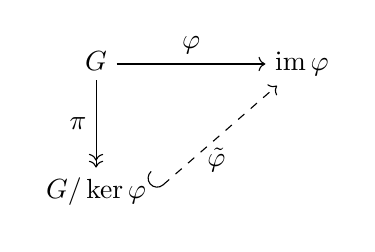
\begin{tikzpicture}
  \matrix (m)
    [
      matrix of math nodes,
      row sep    = 3em,
      column sep = 4em
    ]
    {
      G              & \im \varphi \\
      G/\ker \varphi &             \\
    };
  \path
    (m-1-1) edge [->>] node [left] {$\pi$} (m-2-1)
    (m-1-1.east |- m-1-2)
      edge [->] node [above] {$\varphi$} (m-1-2)
    (m-2-1.east) edge [{Hooks[right,length=0.8ex]}->,
      dashed] node [below] {$\tilde{\varphi}$} (m-1-2);
\end{tikzpicture}
\end{document}